\documentclass[a0paper,portrait]{baposter}

\usepackage{wrapfig}
\usepackage{lmodern}
\usepackage{lipsum,graphicx}
\usepackage[utf8]{inputenc} %unicode support
\usepackage[T1]{fontenc}
\usepackage{tikz}
\usepackage{amsmath}
\usepackage{caption}
\usepackage{algorithm2e}

% allow algorithm2e's float environment inside baposter's minipage-based headerboxes
\makeatletter
\newcommand{\removelatexerror}{\let\@latex@error\@gobble}
\makeatother

\selectcolormodel{cmyk}

\graphicspath{{figures/}{../../slides_soutenance/}{../../images/images_part1/}} % Directories in which figures are stored

\newcommand{\compresslist}{%
\setlength{\itemsep}{0pt}%
\setlength{\parskip}{1pt}%
\setlength{\parsep}{0pt}%
}

\newenvironment{boenumerate}
  {\begin{enumerate}\renewcommand\labelenumi{\textbf\theenumi.}}
  {\end{enumerate}}


\begin{document}

\definecolor{Mycolor1}{HTML}{00FFFF}
\definecolor{Mycolor2}{HTML}{008080}

\begin{poster}
{
grid=false,
headerborder=open, % Adds a border around the header of content boxes
colspacing=1em, % Column spacing
bgColorOne=white, % Background color for the gradient on the left side of the poster
bgColorTwo=white, % Background color for the gradient on the right side of the poster
borderColor=Mycolor1, % Border color
headerColorOne=Mycolor2, % Background color for the header in the content boxes (left side)
headerColorTwo=Mycolor2, % Background color for the header in the content boxes (right side)
headerFontColor=white, % Text color for the header text in the content boxes
boxColorOne=white, % Background color of the content boxes
textborder=rounded, %rectangle, % Format of the border around content boxes, can be: none, bars, coils, triangles, rectangle, rounded, roundedsmall, roundedright or faded
eyecatcher=false, % Set to false for ignoring the left logo in the title and move the title left
headerheight=0.11\textheight, % Height of the header
headershape=rounded, % Specify the rounded corner in the content box headers, can be: rectangle, small-rounded, roundedright, roundedleft or rounded
headershade=plain,
headerfont=\Large\textsf, % Large, bold and sans serif font in the headers of content boxes
%textfont={\setlength{\parindent}{1.5em}}, % Uncomment for paragraph indentation
linewidth=2pt % Width of the border lines around content boxes
}
{}
%
%----------------------------------------------------------------------------------------
%	TITLE AND AUTHOR NAME
%----------------------------------------------------------------------------------------
%
{
\textsf %Sans Serif
{
{Understanding graph representation learning in RL-based logic synthesis}
}
} % Poster title
% {\vspace{0.2em} Add Author Name, Add another author name\\ 
% {\small \vspace{0.7em} School of Enterprise Computing and Digital Transformation, TU Dublin, Tallaght, Dublin, Ireland}} 
{\sf\vspace{0.2em}\\
Hector Kohler, Johannes Lutzeyer, Jesse Read  % Author name
\vspace{0.2em}\\
\small{LIX, Ecole Polytechnique, CNRS, Institut Polytechnique de Paris}
}
{
\includegraphics[width=.25\linewidth]{Kit_logo_web_horizontal/CMJN.png}} % TU Dublin logo


%----------------------------------------------------------------------------------------
%	1. DECISION TREE POLICIES FOR MDPS
%----------------------------------------------------------------------------------------
\headerbox{1. Logic synthesis with and-inverter graphs}{name=introduction,column=0,row=0,span=1}{
Finding the smallest circuit size to encode some Boolean function is key in the chip design industry. This is done in practice with and-inverter graphs (AIGs) which are DAGs where nodes are \textit{AND} gates (in-degrees 2, out-degrees 1) and edge labels are \textit{NOT} signals: any Boolean function can be encoded by such an AIG. Finding the smallest AIG encoding a Boolean function is an instance of minimum circuit size problem which is NP but not yet known to be NP-hard.
\begin{figure}
\begin{subfigure}[b]{0.45\textwidth}
    \centering
    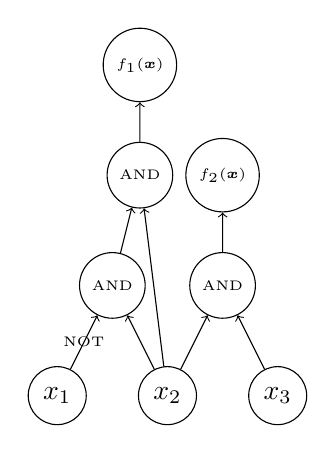
\begin{tikzpicture}[scale=0.7]
        \draw
            (0, 0) node[draw,circle] (0){$x_1$}
            (2, 0) node[draw,circle] (1){$x_2$}
            (4, 0) node[draw,circle] (2){$x_3$}
            (1, 2) node[draw,circle] (3){\tiny AND}
            (3, 2) node[draw,circle] (4){\tiny AND}
            (1.5, 4) node[draw,circle] (5){\tiny AND}
            (3, 4) node[draw,circle] (6){\tiny $f_2(\boldsymbol{x})$}
            (1.5, 6) node[draw,circle] (7){\tiny $f_1(\boldsymbol{x})$};
        \begin{scope}[->]
            \draw (0) to node[] {\tiny NOT} (3);
            \draw (1) to (3);
            \draw (1) to (5);
            \draw (1) to (4);
            \draw (2) to (4);
            \draw (3) to (5);
            \draw (4) to (6);
            \draw (5) to (7);
        \end{scope}
        \end{tikzpicture}
        \subcaption*{$\mathcal{G}_1$: 8 nodes, 4 levels.}
    \end{subfigure}
    \hfill
    \begin{subfigure}[b]{0.45\textwidth}
        \centering
        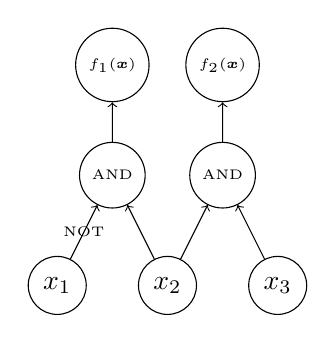
\begin{tikzpicture}[scale=0.7]
        \draw<2->
            (0, 0) node[draw,circle] (0){$x_1$}
            (2, 0) node[draw,circle] (1){$x_2$}
            (4, 0) node[draw,circle] (2){$x_3$}
            (1, 2) node[draw,circle] (3){\tiny AND}
            (3, 2) node[draw,circle] (4){\tiny AND}
            (3, 4) node[draw,circle] (6){\tiny $f_2(\boldsymbol{x})$}
            (1, 4) node[draw,circle] (7){\tiny $f_1(\boldsymbol{x})$};
        \begin{scope}[->]
            \draw<2-> (0) to node[] {\tiny NOT} (3);
            \draw<2-> (1) to (3);
            \draw<2-> (1) to (4);
            \draw<2-> (2) to (4);
            \draw<2-> (3) to (7);
            \draw<2-> (4) to (6);
        \end{scope}
        \end{tikzpicture}
        \subcaption*{$\mathcal{G}_2$: 7 nodes, 3 levels.}
    \end{subfigure}
    \begin{subfigure}
    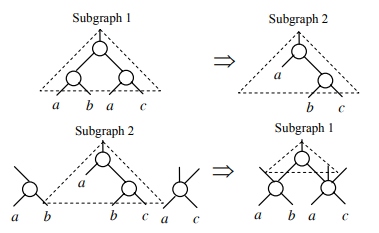
\includegraphics[width=0.7\textwidth]{../aig_rewriting.png}
\end{subfigure}
\end{figure}
\begin{center}
Two functionally equivalent AIGs with different number of nodes for the Boolean function $f(x_1, x_2, x_3) = (\overline{x_1}\land x_2, x_2 \land x_3)$. On the right, one of \textttt{ABC} primitive that apply local AIG modifications while preserving functional equivalence and reducing the number of \textit{AND} nodes~\cite{rewriting}.
\end{center}
}

%----------------------------------------------------------------------------------------
%	2. IMITATION VS DIRECT RL
%----------------------------------------------------------------------------------------
\headerbox{2. AIG reduction as a Markov decision process}{name=how,column=2,row=0,span=2}{
\begin{figure}[h]
  \centering
  \resizebox{\linewidth}{!}{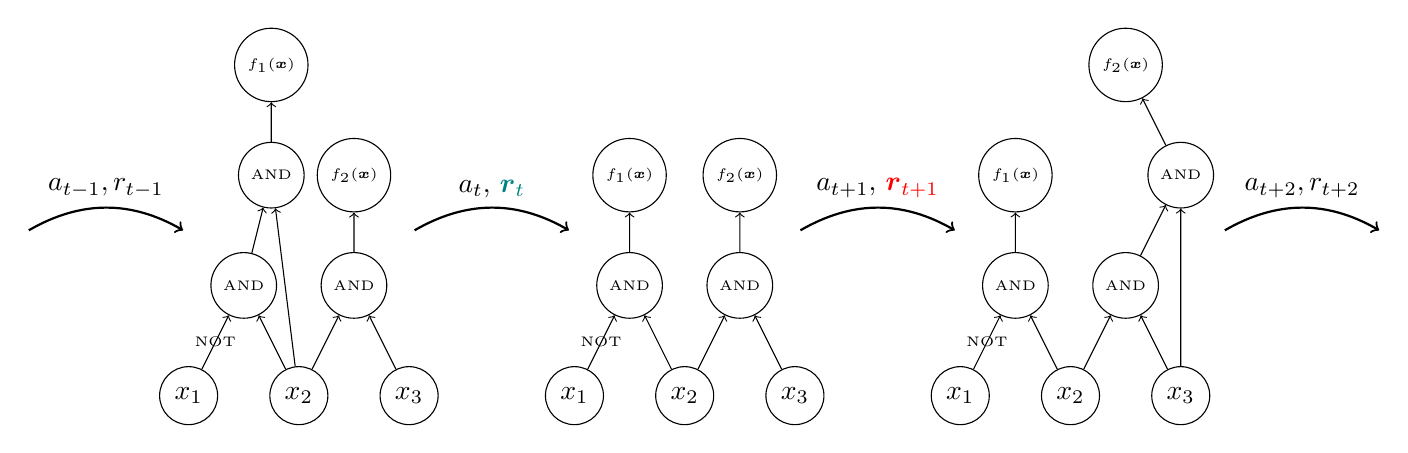
\begin{tikzpicture}[scale=0.7]
        \draw
            (0, 0) node[draw,circle] (0){$x_1$}
            (2, 0) node[draw,circle] (1){$x_2$}
            (4, 0) node[draw,circle] (2){$x_3$}
            (1, 2) node[draw,circle] (3){\tiny AND}
            (3, 2) node[draw,circle] (4){\tiny AND}
            (1.5, 4) node[draw,circle] (5){\tiny AND}
            (3, 4) node[draw,circle] (6){\tiny $f_2(\boldsymbol{x})$}
            (1.5, 6) node[draw,circle] (7){\tiny $f_1(\boldsymbol{x})$};
        \begin{scope}[->]
            \draw (0) to node[] {\tiny NOT} (3);
            \draw (1) to (3);
            \draw (1) to (5);
            \draw (1) to (4);
            \draw (2) to (4);
            \draw (3) to (5);
            \draw (4) to (6);
            \draw (5) to (7);
        \end{scope}
        \draw
            (7, 0) node[draw,circle] (8){$x_1$}
            (9, 0) node[draw,circle] (9){$x_2$}
            (11, 0) node[draw,circle] (10){$x_3$}
            (8, 2) node[draw,circle] (11){\tiny AND}
            (10, 2) node[draw,circle] (12){\tiny AND}
            (10, 4) node[draw,circle] (13){\tiny $f_2(\boldsymbol{x})$}
            (8, 4) node[draw,circle] (14){\tiny $f_1(\boldsymbol{x})$};
        \begin{scope}[->]
            \draw (8) to node[] {\tiny NOT} (11);
            \draw (9) to (11);
            \draw (9) to (12);
            \draw (10) to (12);
            \draw (11) to (14);
            \draw (12) to (13);
        \end{scope}
        \draw[thick, ->] (4.1,3) to[bend left=30] node[midway, above] {$a_t$, \textcolor{teal}{$\boldsymbol{r}_t$}} (6.9,3);
        \draw[thick, ->] (-2.9,3) to[bend left=30] node[midway, above] {$a_{t-1}, r_{t-1}$} (-0.1,3);
        \draw[thick, ->] (18.8,3) to[bend left=30] node[midway, above] {$a_{t+2}, r_{t+2}$} (21.6,3);
        \draw[thick, ->] (11.1,3) to[bend left=30] node[midway, above] {$a_{t+1}$, \textcolor{red}{$\boldsymbol{r}_{t+1}$}} (13.9,3);
        \draw
            (14, 0) node[draw,circle] (8){$x_1$}
            (16, 0) node[draw,circle] (9){$x_2$}
            (18, 0) node[draw,circle] (10){$x_3$}
            (15, 2) node[draw,circle] (11){\tiny AND}
            (17, 2) node[draw,circle] (12){\tiny AND}
            (17, 6) node[draw,circle] (13){\tiny $f_2(\boldsymbol{x})$}
            (18, 4) node[draw,circle] (99){\tiny AND}
            (15, 4) node[draw,circle] (14){\tiny $f_1(\boldsymbol{x})$};
        \begin{scope}[->]
            \draw (8) to node[] {\tiny NOT} (11);
            \draw (9) to (11);
            \draw (9) to (12);
            \draw (10) to (99);
            \draw (10) to (12);
            \draw (12) to (99);
            \draw (11) to (14);
            \draw (99) to (13);
        \end{scope}
  \end{tikzpicture}}
  \caption{A trajectory in a generic MDP for AIG reduction, on AIGs of the Boolean function $f(x_1, x_2, x_3) = (\bar{x_1}\land x_2,\ x_2 \land x_3)$. A policy gets more reward for reducing the number of \textit{AND} nodes in an AIG. Most reinforcement learning (RL) and other machine learning-based search for logic synthesis~\cite{rl-gnn1,rl-logic1,flow-bandits} that efficiently reduce AIGs act at this granularity: each action is one \texttt{ABC} primitive applied to the whole graph. Those primitives preserve functional equivalence by construction, so every state reachable from $\mathcal{G}_0$ still computes $f$. DAG generative models have been used to generate reduced AIGs when given some AIGs but those fail completely~\cite{graphbench}.}
\end{figure}
}

\headerbox{3. Graph representation and reinforcement learning~\citet{rl-gnn1}}{name=ibmdp,column=0,below=introduction,span=2}{
We train \textbf{tuned} PPO agents to reduce some standards AIGs encoding different Boolean functions. We focus on performance differences between GCN policies and graph statistics (current \# nodes, \# edges, last few graph edits taken, current time steps) policies.
\begin{figure}[t]
  \centering
  
\includegraphics[width=\linewidth]{figures/fig_gcn_main.pdf}
  \caption{PPO on the ten benchmarks from~\citet{rl-gnn1} with five observation encoders, each tuned (cf. appendix~\ref{app:rl-hp} for more details). (a) AND count averaged over the ten
  benchmarks; (b) change in final AND count against the no-GCN policy, per
  benchmark and pooled over the ten (\emph{all 10}), the grey band being the
  no-GCN policy's own spread over its five seeds; (c) the pooled change against
  the parameters the encoder adds to the policy. All intervals are 95\%
  bootstrap confidence intervals over five seeds.}
  \label{fig:rl-main}
\end{figure}
}
\headerbox{4. Final AIG sizes}{name=triad,column=2,below=how,span=1}{
\begin{table}[t]
  \centering\small
  \caption{Mean AND count after $H=20$ \texttt{ABC} primitives, over the five
  seeds of each configuration's best hyper-parameter cell, $\pm$ one standard
  deviation across those seeds. \emph{Starting nodes} is the AND count of the benchmark
  before any primitive is applied; \texttt{resyn2} is deterministic and has no
  spread. AIGs are ordered by input size.}
  \label{tab:rl-ands}
  % mean final AND count over the 5 seeds of the best cell, $\pm$ s.d. over those seeds
\begin{tabular}{lrrrrrrr}
\toprule
benchmark & input & no GCN (MLP) & GCN small & GCN medium & GCN large & GCN v.\,large & \texttt{resyn2} \\
\midrule
C1355 & 504 & 389\,{\tiny$\pm$3} & \textbf{387}\,{\tiny$\pm$1} & \textbf{387}\,{\tiny$\pm$0} & \textbf{387}\,{\tiny$\pm$1} & \textbf{387}\,{\tiny$\pm$0} & 390 \\
dalu & 1740 & 1008\,{\tiny$\pm$9} & 1006\,{\tiny$\pm$6} & \textbf{1001}\,{\tiny$\pm$3} & 1006\,{\tiny$\pm$6} & 1005\,{\tiny$\pm$2} & 1052 \\
C5315 & 1773 & 1303\,{\tiny$\pm$43} & 1287\,{\tiny$\pm$8} & 1283\,{\tiny$\pm$2} & \textbf{1282}\,{\tiny$\pm$6} & 1283\,{\tiny$\pm$5} & 1309 \\
C7552 & 2074 & 1371\,{\tiny$\pm$12} & 1372\,{\tiny$\pm$10} & \textbf{1367}\,{\tiny$\pm$11} & 1369\,{\tiny$\pm$5} & 1369\,{\tiny$\pm$10} & 1455 \\
apex1 & 2124 & 1066\,{\tiny$\pm$7} & 1064\,{\tiny$\pm$11} & 1074\,{\tiny$\pm$4} & 1070\,{\tiny$\pm$4} & \textbf{1063}\,{\tiny$\pm$14} & 1179 \\
k2 & 2190 & 1049\,{\tiny$\pm$26} & \textbf{1015}\,{\tiny$\pm$32} & 1019\,{\tiny$\pm$27} & 1027\,{\tiny$\pm$21} & 1030\,{\tiny$\pm$36} & 1194 \\
C6288 & 2337 & \textbf{1870}\,{\tiny$\pm$0} & \textbf{1870}\,{\tiny$\pm$0} & \textbf{1870}\,{\tiny$\pm$0} & \textbf{1870}\,{\tiny$\pm$0} & \textbf{1870}\,{\tiny$\pm$0} & 1870 \\
i10 & 2675 & 1715\,{\tiny$\pm$13} & \textbf{1700}\,{\tiny$\pm$3} & 1705\,{\tiny$\pm$9} & 1702\,{\tiny$\pm$3} & 1702\,{\tiny$\pm$6} & 1829 \\
bc0 & 3501 & 1512\,{\tiny$\pm$46} & 1485\,{\tiny$\pm$59} & 1481\,{\tiny$\pm$31} & 1484\,{\tiny$\pm$28} & \textbf{1455}\,{\tiny$\pm$13} & 1713 \\
mainpla & 6359 & 2318\,{\tiny$\pm$37} & 2306\,{\tiny$\pm$14} & \textbf{2298}\,{\tiny$\pm$11} & 2305\,{\tiny$\pm$23} & 2307\,{\tiny$\pm$14} & 2476 \\
\midrule
mean AND\,/\,input & & 0.596 & 0.592 & 0.592 & 0.592 & 0.591 & 0.628 \\
\bottomrule
\end{tabular}

\end{table}
}

% %----------------------------------------------------------------------------------------
% %	4. GROUND TRUTH: OPTIMAL TREES ARE KNOWN
% %----------------------------------------------------------------------------------------
\headerbox{5. Why don't graph representation significantly improve RL-based logic synthesis?}{name=optimal,column=0,below=ibmdp,span=2}{
\begin{figure}[t]
  \centering
  \resizebox{\linewidth}{!}{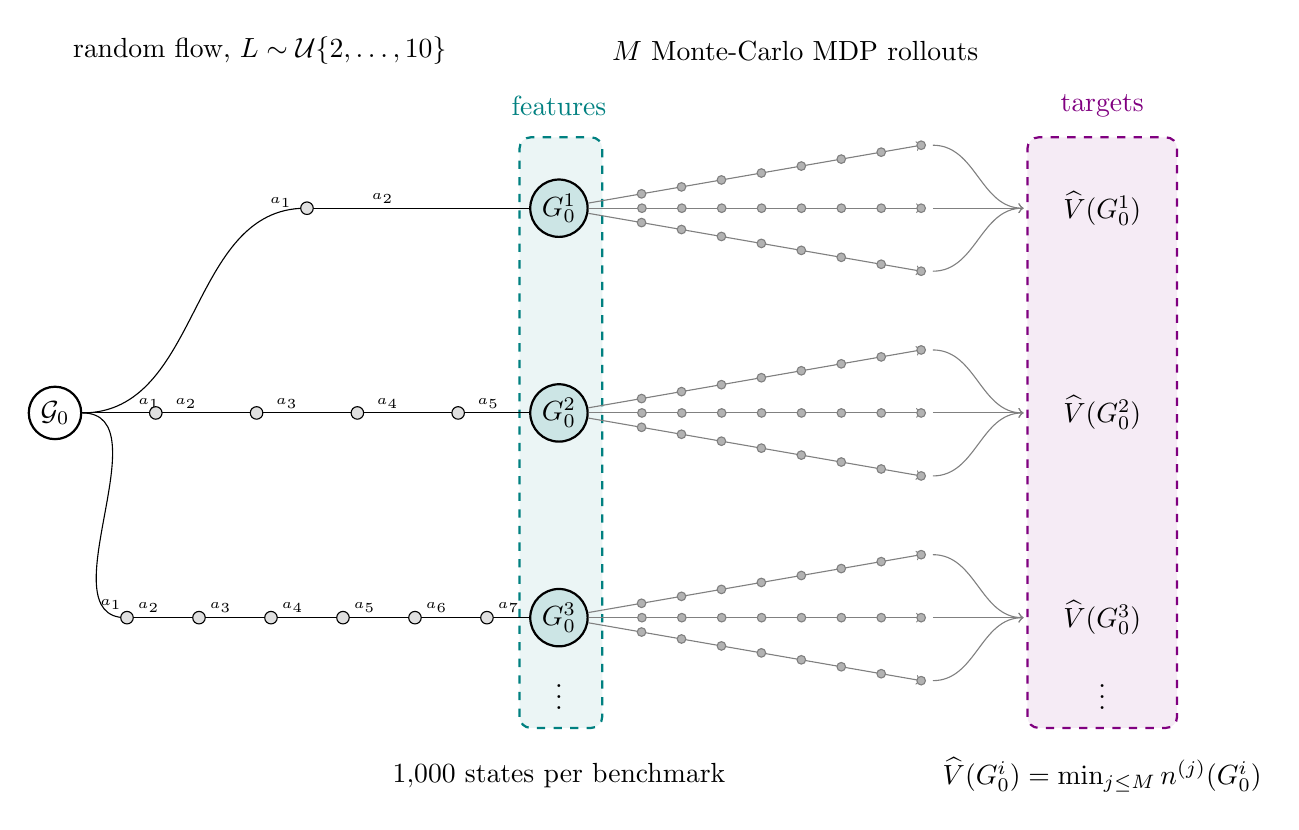
\begin{tikzpicture}[
      aig/.style={draw,circle,inner sep=1.6pt,fill=black!12},
      state/.style={draw,thick,circle,inner sep=1.6pt,fill=teal!20},
      leaf/.style={draw=gray,circle,inner sep=1.1pt,fill=gray!60},
      act/.style={font=\tiny,inner sep=1.5pt},
      roll/.style={gray,->},
      panel/.style={draw,dashed,rounded corners,thick}]
    % the two columns of the supervised dataset, drawn first so they sit behind
    \draw[panel,teal,fill=teal!8]     (5.9,-4.0) rectangle (6.95,3.5);
    \draw[panel,violet,fill=violet!8] (12.35,-4.0) rectangle (14.25,3.5);
    \node[teal] at (6.4,3.9) {features};
    \node[violet] at (13.3,3.9) {targets};
    \node[draw,thick,circle,inner sep=2pt] (g0) at (0,0) {$\mathcal{G}_0$};
    % states: a uniformly random flow of length L, one row per length
    \foreach \y/\n/\i in {2.6/2/1, 0/5/2, -2.6/7/3}{
      \pgfmathsetmacro{\dx}{6.4/\n}
      \pgfmathtruncatemacro{\m}{\n-1}
      \draw[->] (g0) to[out=0,in=180] node[act,above,pos=0.92] {$a_1$} ({\dx},\y);
      \foreach \k in {2,...,\n}{
        \pgfmathsetmacro{\xa}{(\k-1)*\dx}
        \draw[->] ({\xa},\y) -- node[act,above,pos=0.3] {$a_{\k}$} ({\xa+\dx},\y);}
      \foreach \k in {1,...,\m}{\node[aig] at ({\k*\dx},\y) {};}
      \node[state] (s\i) at (6.4,\y) {$G_0^\i$};
      \coordinate (v\i) at (12.3,\y);
      \node at (13.3,\y) {$\widehat{V}(G_0^\i)$};
      % M rollouts of eight uniformly random primitives
      \foreach \o in {0.8,0,-0.8}{
        \draw[roll] (s\i) -- ({11},{\y+\o})
          \foreach \p in {0.16,0.28,...,0.88} {node[leaf,pos=\p]{}};
        \node[leaf] at (11,{\y+\o}) {};
        \draw[roll] (11.15,{\y+\o}) to[out=0,in=180] (v\i);}
    }
    \node at (2.6,4.6) {random flow, $L\sim\mathcal{U}\{2,\dots,10\}$};
    \node at (9.4,4.6) {$M$ Monte-Carlo MDP rollouts};
    \node at (6.4,-3.5) {$\vdots$};
    \node at (13.3,-3.5) {$\vdots$};
    \node at (6.4,-4.6) {$1{,}000$ states per benchmark};
    \node at (13.3,-4.6) {$\widehat{V}(G_0^i) = \min_{j\leq M} n^{(j)}(G_0^i)$};
  \end{tikzpicture}}
  \caption{Building the value prediction dataset. Applying to the benchmark $\mathcal{G}_0$ a uniformly random flow $a_1,\dots,a_L$ of \texttt{ABC} primitives gives a state $G_0^i$, an AIG functionally equivalent to $\mathcal{G}_0$ but in general of a different size; the length $L$ of the flow is itself drawn at random, so the states sit at varying distances from $\mathcal{G}_0$. The target of a state is the smallest AND count $\widehat{V}(G_0^i)$ reached by $M=100$ independent rollouts of eight further uniformly random primitives from it. The two dashed columns are the resulting supervised regression dataset: each state is an input, stored both as an \texttt{.aig} file and as the statistics $x_\mathcal{G}$ of section~\ref{sec:features} so that every model class of section~\ref{sec:bounds} sees the same states, and $\widehat{V}(G_0^i)$ is its target. The procedure is repeated for $1{,}000$ states per benchmark, on ten AIGs and ten seeds.}
  \label{fig:dataset}
\end{figure}
Computing $V^\star$ exactly is out of reach: the tree of flows over the five primitives of section~\ref{sec:method} has $5^H$ leaves, and every edge of it costs one \texttt{ABC} call on the full circuit.
We therefore estimate it by sampling both the states and the continuations from them, as shown in figure~\ref{fig:dataset}.
A state is the AIG obtained by applying to the benchmark $\mathcal{G}_0$ a uniformly random flow of length $L\sim\mathcal{U}\{2,\dots,10\}$; we draw $1{,}000$ such states per benchmark and store each one both as an \texttt{.aig} file and as the statistics $x_\mathcal{G}$ of section~\ref{sec:features}, so that every model class of section~\ref{sec:bounds} is evaluated on exactly the same states and the same targets.
From each state $s$ we then run $M = 100$ independent rollouts of $8$ further uniformly random primitives and keep the best AND count reached, $\widehat{V}(s) = \min_{j \leq M} n^{(j)}(s)$, an upper bound on the minimum over the $5^8$ flows of length eight that approaches it from above as $M$ grows.
A key difference to $V^\star$ should be kept in mind: $\widehat{V}$ truncates the horizon at eight steps instead of the $H=20$ of the reinforcement learning experiments, so our targets approximate the value of an eight-step-to-go problem, and the bounds of section~\ref{sec:bounds} are lower bounds on the error of predicting \emph{that} quantity.
The procedure is repeated with ten seeds per benchmark on the same ten AIGs as in section~\ref{sec:rl-exp}, and the figures of this section report over those ten repetitions.
The sampler is degenerate on two of them, reaching only two distinct values of $\widehat{V}$ on \texttt{C6288} and six on \texttt{C1355}: we exclude \texttt{C6288} and report over the remaining nine benchmarks, flagging \texttt{C1355} wherever it appears.

}
\headerbox{6. 1-WL representation for AIGs~\citet{graphtester}}{name=asym,column=2,below=triad,span=1}{
\begin{figure}[t]
  \centering
  
\includegraphics[width=0.9\linewidth]{figures/fig_value_bounds.pdf}
  \caption{Best error (a) and best ranking (b) achievable by each model class on
  $\widehat{V}$, over nine benchmarks and ten dataset seeds. Each class is replaced
  by the optimal predictor for the information it can distinguish, so the value
  shown cannot be beaten by any model in that class. $^{*}$\texttt{C1355} has
  only six distinct targets.}
  \label{fig:bounds}
\end{figure}
}
%----------------------------------------------------------------------------------------
%	5. RL FAILS, EVEN ASYMMETRIC RL
%----------------------------------------------------------------------------------------
\headerbox{7. Preliminary results for AIG-specific models for value predictions}{name=results,column=0,below=optimal,span=1}{
\begin{figure}[h]
  \centering
  
\includegraphics[width=\linewidth]{figures/fig_training_curves.pdf}
  \caption{Validation error over training for tuned AIG-specific models~\cite{deepgate} and generic graph representation models}
  \label{fig:curves}
\end{figure}
}
\headerbox{8. Additional results}{name=results,column=0,below=optimal,span=1}{
Figure~\ref{fig:depth} plots the message passing bound of section~\ref{sec:bounds} against the number of refinement iterations $k$, for the four views of the AIG bounded there.
The bound moves by at most $1.1\times10^{-3}$ between $k = 1$ and $k = 50$, and labeling edges with direction or with the complement bit changes it by less than $10^{-6}$, so neither deeper refinement nor a richer view of the graph brings a message passing network closer to $\widehat{V}$.

\begin{figure}[h]
  \centering
  
\includegraphics[width=\linewidth]{figures/fig_mpnn_depth.pdf}
  \caption{The MPNN bound as a function of depth $k$.}
  \label{fig:depth}
\end{figure}
\begin{figure}[h]
  \centering
  
\includegraphics[width=\linewidth]{figures/fig_gcn_ex_size.pdf}
  \caption{Reduction against the MLP as a function of input circuit size on
  \texttt{ex200}--\texttt{ex299}. Line: mean over size quartiles.}
  \label{fig:rl-ex-size}
\end{figure}
}
\headerbox{9. Future work}{name=results,column=0,below=optimal,span=1}{
\begin{itemize}
    \item Extend our analysis to non 1-WL representation (some AIG-specific models might not be 1-WL)
    \item Extend our analysis to larger AIG primitive operations (the standard \texttt{ABC} software has way more than 5 primitive implemented but there is no search method considering the complete action space available). More actions in the AIG reduction MDP means more varied states which is where graph representation learning could bring significantly
\end{itemize}
\bibliographystyle{plainnat}
\bibliography{neurips_2026}
}

% %----------------------------------------------------------------------------------------
% %	6. ABLATING PARTIAL OBSERVABILITY
% %----------------------------------------------------------------------------------------
% \headerbox{6. Ablation: removing partial observability}{name=ablation,column=0,below=results,span=2,above=bottom}{
% \begin{center}
% \begin{tabular}{cc}
% \scalebox{0.95}{\begin{tikzpicture}[
%         decision/.style={circle, draw, thick, fill=blue!20, text width=2.5em, text centered, minimum height=2.5em, font=\small},
%         edge_label/.style={font=\footnotesize, midway}
%     ]
%         % Classification task as a downstream MDP
%         \draw[fill=green!40] (0, 0) rectangle (1,2);
%         \draw[fill=red!40] (1, 0) rectangle (2,2);
%         \draw[draw, thick] (0,0) grid (2,2);
%         \draw[thick, ->] (0,0) -- (2.5,0) node[right] {$x$};
%         \draw[thick, ->] (0,0) -- (0,2.5) node[above] {$y$};
%         \foreach \x in {0,1,2} {
%             \draw[thick] (\x,0) -- (\x,-0.1) node[below] {$\x$};
%         }
%         \foreach \y in {0,1,2} {
%             \draw[thick] (0,\y) -- (-0.1,\y) node[left] {$\y$};
%         }

%         % Optimal depth-1 tree classifier
%         \node[decision] (croot) at (5,2) {$x \leq 1$};
%         \node[rectangle, draw, thick, fill=green!40, text width=2em, text centered, rounded corners, minimum height=2em, font=\small] (cleft) at (4,0) {};
%         \node[rectangle, draw, thick, fill=red!40, text width=2em, text centered, rounded corners, minimum height=2em, font=\small] (cright) at (6,0) {};
%         \draw[->] (croot) -- (cleft) node[edge_label, above left] {True};
%         \draw[->] (croot) -- (cright) node[edge_label, above right] {False};
%     \end{tikzpicture}}
% &
% \includegraphics[width=0.45\linewidth]{tree_distributions_merged.pdf}
% \end{tabular}
% \end{center}
% \small
% When the downstream MDP has uniform transitions---e.g. it encodes a \textbf{classification task} (left)---the POIBMDP is fully observable.
% Standard RL then \textbf{consistently} trains optimal decision trees (right): \textbf{partial observability is the culprit}.
% }

% %----------------------------------------------------------------------------------------
% %	7. TAKEAWAYS
% %----------------------------------------------------------------------------------------
% \headerbox{7. Takeaways}{name=takeaways,column=2,below=results,span=1,above=bottom}{
% \begin{itemize}\compresslist
%     \item Training a decision tree policy directly with RL $\equiv$ solving a POMDP with a \textbf{deterministic memoryless} policy: a deadly triad.
%     \item Even dedicated asymmetric RL cannot consistently retrieve the known optimal depth-1 tree of a $2\times2$ grid world.
%     \item Remove partial observability and the same algorithms succeed consistently.
% \end{itemize}
% \medskip

% \small Code: \texttt{github.com/KohlerHECTOR/poibmdps}
% }
\end{poster}

\end{document}
